%%\section{Histórico de Evolução}
%-------------------------------------------------------------------------------------- Início
\begin{frame}[allowframebreaks,fragile,t]{Histórico do Rails}
  \begin{itemize}
  	\item Rails é um \textit{framework} para construção de aplicações web
    \item David Heinemeier Hanson \alert{derivou} o Rails a partir do BaseCamp --
      uma ferramenta de gestão de projetos da empresa 37Signals.
    \begin{itemize}
	\item a primeira versão de código aberto (em inglês: \textit{open source})foi liberada em 
	  julho de 2004.
	\item mas direitos para que outros desenvolvedores \alert{colaborassem} com o projeto foram liberadosw
	  em fevereiro de 2005.
    \end{itemize}
    \item Em agosto de 2006, o Ruby on Rails atingiu um \alert{marco importante} quando a Apple dicidiu
      distribuído juntamente com a versão do seu sistema operacional Mac OS X v10.5 "Leopard"
    \begin{itemize}
     \item nesse mesmo no o Rails começou a ganhar muita atenção da comunidade de desenvolvimento web.
    \end{itemize}
    \item Rails é utilizado por diversas companhias, como por exemplo:
    \begin{itemize}
     \item Airbnb, BaseCamp, Disney, GitHub, Hulu, Kickstarter, Shopify e Twitter.
    \end{itemize}

  \end{itemize}

  \begin{figure}[h]
    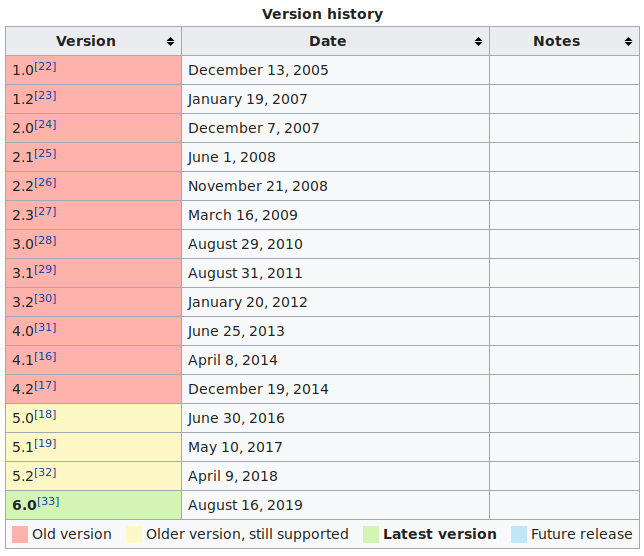
\includegraphics[scale=0.3]{imagens/rails-history.png}  
  \end{figure}
\end{frame}
